\FloatBarrier
\section{Experiments}
\label{sec:llm}
\label{sec:results}

\subsection{Protocol}
\label{sec:setup}

We report four evidence layers. First, fixed-history replay crosses scripted design
policies with ordinary, block-aware and component-aware GP readers, where a reader maps a
completed visible history to a recommendation. Each reader receives a copy of the same
accepted and completed history, so changing the reader cannot change the evidence it reads.
Second, the frozen Phase~4 protocol runs closed-loop model agents on reserved sites. Its
primary matrix crosses Luna with bare, design-aid, inference-aid and combined interfaces on
\textsc{Optimise}: 56 sites, two provider generation seeds and 448 episodes. Prespecified
secondary matrices add 96 Sol episodes, 192 Luna episodes on \textsc{Sanity} and
\textsc{Transfer}, 96 Luna episodes comparing terminal-only and within-cycle access, and 96
prompt-variant episodes, for 928 total. Third, after the primary analysis was frozen, a
separately registered robustness extension reruns all four Luna interfaces on 16 fresh
sites, two provider generations and noise multipliers $0.5,1,2$, for 384 further episodes.
Fourth, a prospective post-primary model extension crosses Luna, DeepSeek V4.1 Flash and
Qwen 3.8 27B with bare and inference-aid interfaces on the same 24 \textsc{Optimise} sites
and two generation seeds, for 288 episodes.

A site, rather than an API completion, is the inferential unit. We average the two provider
generations within each site, form paired differences, and use a 10,000-resample site
bootstrap for percentile 95\% intervals. The primary three tool-minus-bare comparisons use
Holm family-wise correction. Named secondary families use Benjamini--Hochberg adjustment;
the model extension separately adjusts its three within-model contrasts and six same-arm
model contrasts. Model-format failures, infeasible submissions and early stopping remain
outcomes; only transport failures are retried with the same identity. The 928-episode run
and 288-episode extension both have no missing or duplicate cells. Appendix~
\ref{app:phase4-protocol} gives hashes, site ranges, API metadata and the distinction
between confirmatory, secondary and post-primary analyses.

\subsection{Fixed histories separate allocation from evidence use}

On held-out Phase~3 sites, the range across scripted design sources is $0.01718$ regret,
the range across deployable readers is $0.00619$, and the design--reader interaction RMS is
$0.00209$. The relative size is task dependent: the design range is largest on
\textsc{Transfer} ($0.04727$), whereas on \textsc{Sanity} the reader range exceeds the
design range. This supports treating allocation and history reading as separate capabilities;
it does not support a universal claim that one dominates. The block-aware reader also fails
to beat the ordinary GP on its independent calibration set (paired normalized-regret
improvement $-0.0112$, SE $0.0095$, 24 pairs), so we retain it as a structural diagnostic
rather than designate it a stronger baseline. Figure~\ref{fig:phase5-mechanisms} places the
executed design, reader crossing, feedback contrast and evaluator check on one scale-aware
mechanism summary.

\begin{figure*}[t]
\centering
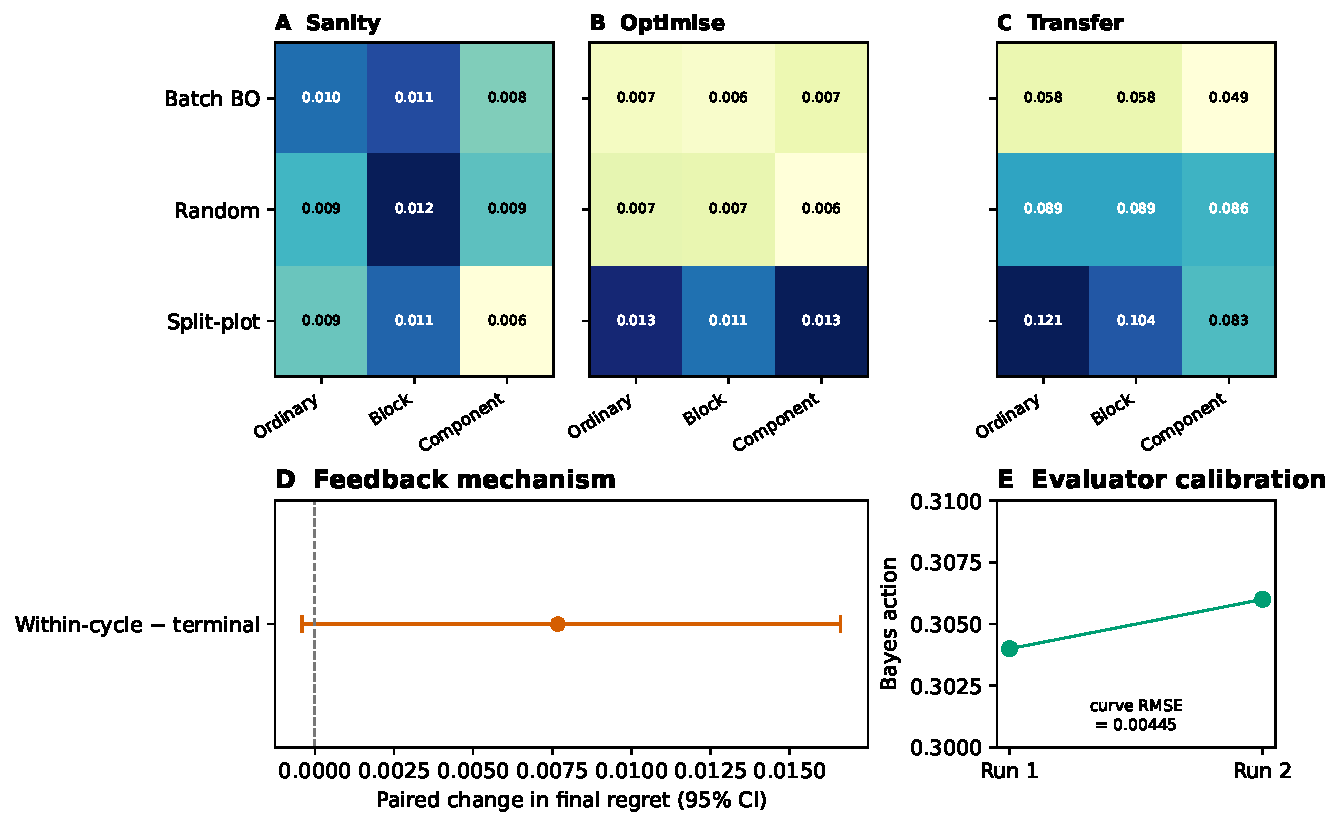
\includegraphics[width=\textwidth]{figures/fig3_phase5_mechanisms.pdf}
\caption{Mechanism checks behind the endpoint comparisons. (A--C) Fixed-history
design--reader crossings for \textsc{Sanity}, \textsc{Optimise} and \textsc{Transfer}; rows
change the executed scripted design and columns change only evidence use. Each cell averages
eight held-out sites. Color scales are independent across panels and the annotations give
mean realized regret. (D) Registered paired effect of within-cycle access; positive is
worse. (E) Two independent factorized evaluator runs select nearly identical Bayes actions;
the annotation reports response-curve disagreement.}
\label{fig:phase5-mechanisms}
\end{figure*}

\begin{table*}[t]
\centering\small
\setlength{\tabcolsep}{4.5pt}
\begin{tabular}{@{}llrrll@{}}
\toprule
Policy & Reader / aid & Sites $\times$ repeats & Mean regret & $\Delta$ vs. bare [95\% CI] & adjusted $p$ \\
\midrule
Random spread & ordinary GP & 8 $\times$ 1 & 0.0072 & descriptive & --- \\
Split-plot DOE & ordinary GP & 8 $\times$ 1 & 0.0128 & descriptive & --- \\
Batch BO & ordinary GP & 8 $\times$ 1 & 0.0066 & descriptive & --- \\
\addlinespace
Luna & none & 56 $\times$ 2 & 0.0128 & reference & --- \\
Luna & design & 56 $\times$ 2 & 0.0129 & +0.0002 [-0.0030, +0.0032] & 1.000 \\
Luna & inference & 56 $\times$ 2 & 0.0108 & -0.0020 [-0.0052, +0.0013] & 0.727 \\
Luna & both & 56 $\times$ 2 & 0.0126 & -0.0002 [-0.0037, +0.0033] & 1.000 \\
\addlinespace
Sol & none & 24 $\times$ 2 & 0.0030 & reference & --- \\
Sol & inference & 24 $\times$ 2 & 0.0035 & +0.0005 [-0.0006, +0.0017] & 0.381 \\
\bottomrule
\end{tabular}
\caption{Final simple regret on \textsc{Optimise} (lower is better). Scripted rows are fixed-history reader replays on eight Phase~3 sites and are descriptive; they are included as reference points, not tested against the independently sampled model runs. Phase~4 model contrasts average two provider generations within each site before inference. Luna tool contrasts use Holm correction across the three preregistered comparisons; the Sol replication uses the prespecified secondary-family adjustment.}
\label{tab:phase4-main}
\end{table*}


\subsection{Standard aids do not reliably reduce final regret}

Table~\ref{tab:phase4-main} contains the preregistered primary comparisons. For Luna, the
design-aid difference is $+0.00016$ (95\% CI $[-0.00299,0.00321]$), inference aid is
$-0.00196$ ($[-0.00520,0.00133]$), and both aids are $-0.00023$
($[-0.00365,0.00326]$). None is significant after Holm correction. Sol reaches lower
absolute regret than Luna on its independently sampled sites, but its inference aid also
does not improve the bare arm: $+0.00053$ ($[-0.00055,0.00173]$), adjusted $p=0.381$.
Absolute model levels are descriptive because the two models use different reserved sites;
the registered inference concerns each paired aid contrast.

The tools were available and often followed. In the Luna primary matrix, the geometric
adoption rate is $0.33$ for design-only and $0.31$ with both aids; inference recommendations
are adopted at rates $0.88$ and $0.94$. The null effects therefore do not arise from complete
non-use. They show that these particular tools, delivery format and agents do not reliably
convert adoption into lower endpoint regret.

\subsection{Inference-aid value is model dependent}

\begin{table}[t]
\centering
\small
\setlength{\tabcolsep}{4.5pt}
\begin{tabular}{lrrrr}
\toprule
Model & Bare & Inference & $\Delta$ [95\% CI] & BH $p$ \\
\midrule
Luna & 0.0107 & 0.0106 & -0.0001 [-0.0065, +0.0065] & 0.975 \\
DeepSeek V4.1 Flash & 0.0112 & 0.0081 & -0.0031 [-0.0070, +0.0007] & 0.186 \\
Qwen 3.8 27B & 0.0242 & 0.0097 & -0.0146 [-0.0201, -0.0091] & $<0.001$ \\
\bottomrule
\end{tabular}
\caption{Prospective post-primary model extension on \textsc{Optimise}. Values are mean final simple regret (lower is better); $\Delta$ is inference minus bare. Each arm contains 24 common sites and two generation seeds, averaged within site before the 10,000-resample bootstrap. BH correction covers the three within-model contrasts.}
\label{tab:phase5-model-extension}
\end{table}


Table~\ref{tab:phase5-model-extension} reports the prospective extension, which changes
the interpretation of the earlier nulls. On the same 24
sites, inference minus bare final regret is $-0.00010$ for Luna (95\% CI
$[-0.00647,0.00646]$, BH $p=0.975$), $-0.00306$ for DeepSeek V4.1 Flash
($[-0.00698,0.00070]$, BH $p=0.186$), and $-0.01456$ for Qwen 3.8 27B
($[-0.02005,-0.00914]$, BH $p<0.001$). Thus the aid produces a clear endpoint improvement
for Qwen, a directionally favorable but uncertain estimate for DeepSeek, and no detectable
change for Luna under these interfaces.

Qwen's bare regret exceeds both Luna's and DeepSeek's after adjustment, whereas none of the
three pairwise model contrasts is significant under the inference interface. This pattern
does not rank the base models: it shows that the measured bare-model gap is absent when the
same inference aid is supplied. Cumulative regret also falls within every model (site-
bootstrap 95\% intervals exclude zero), but this secondary endpoint mixes experimental
allocations with stopping behavior. Inference recommendations are adopted on $0.87$, $0.66$
and $0.48$ of eligible rounds for Luna, DeepSeek and Qwen, respectively, so adoption rate
alone does not explain the endpoint effect.

\begin{table}[t]
\centering\small
\setlength{\tabcolsep}{4pt}
\begin{tabular}{@{}lrrrl@{}}
\toprule
Contrast & sites & $\Delta$ regret & 95\% CI & adjusted $p$ \\
\midrule
Luna, T1: inference $-$ bare & 24 & -0.0008 & [-0.0053, +0.0037] & 0.722 (BH) \\
Luna, T4: inference $-$ bare & 24 & +0.0114 & [-0.0017, +0.0287] & 0.313 (BH) \\
Luna, within-cycle $-$ terminal-only & 24 & +0.0077 & [-0.0004, +0.0166] & 0.085 (BH) \\
Luna, 0.5$\times$ noise: design $-$ bare & 16 & +0.0113 & [+0.0053, +0.0184] & 0.010 (BH) \\
Luna, 2$\times$ noise: design $-$ bare & 16 & +0.0048 & [-0.0047, +0.0131] & 0.605 (Holm) \\
Luna, 2$\times$ noise: inference $-$ bare & 16 & -0.0067 & [-0.0155, +0.0012] & 0.374 (Holm) \\
Luna, 2$\times$ noise: both $-$ bare & 16 & -0.0040 & [-0.0116, +0.0032] & 0.605 (Holm) \\
\bottomrule
\end{tabular}
\caption{Held-out secondary and robustness contrasts (positive values are worse). The half-noise design-aid contrast is the only listed interval that excludes zero.}
\label{tab:phase4-secondary}
\end{table}


Task and feedback extensions in Table~\ref{tab:phase4-secondary} remain uncertain. The
inference-aid point estimate is slightly favorable on \textsc{Sanity} and unfavorable on
\textsc{Transfer}; both intervals cross zero after the prespecified correction. Allowing
Luna to inspect time-appropriate within-cycle measurements changes its actions and increases
API use, but the final-regret difference against terminal-only access is $+0.00768$
($[-0.00041,0.01662]$, adjusted $p=0.085$). Under the present synchronous action space,
committed treatments cannot change and the next batch receives terminal outcomes anyway.
Interim observation can therefore update an interim recommendation, but it has no guaranteed
path to improve the next design. Testing value from inspection requires a consequential
action such as staggered release, early termination or treatment modification.

\subsection{Robustness changes the conclusion only at lower noise}

The fresh adaptive extension asks whether observation noise changes later designs and
recommendations, which fixed-policy rescoring cannot test. At twice the registered noise,
all three tool-minus-bare intervals cross zero (Table~\ref{tab:phase4-secondary}), matching
the primary conclusion. The prespecified secondary family gives a different result at half
noise: design aid increases regret by $0.01133$ (95\% CI $[0.00530,0.01842]$, adjusted
$p=0.0096$). Inference-only and combined aids at half noise, all one-noise contrasts, and
the registered $2\times$ versus $1\times$ interactions are not significant. We therefore
report a bounded conclusion: the tested tools show no reliable improvement, and one
lower-noise condition shows harm; the evidence does not establish a universal direction
across models, domains or tool implementations.

\subsection{Transfer is evaluated after the price shock}

\begin{table}[t]
\centering\small
\begin{tabular}{@{}lrrr@{}}
\toprule
Condition & sites $\times$ repeats & pre-shock & post-shock \\
\midrule
Luna bare & 24 $\times$ 2 & 0.0602 $\pm$ 0.0054 & 0.0681 $\pm$ 0.0095 \\
Luna inference & 24 $\times$ 2 & 0.0716 $\pm$ 0.0074 & 0.1133 $\pm$ 0.0140 \\
\midrule
Inference $-$ bare (post-shock) & 24 sites & \multicolumn{2}{r}{+0.0452 [+0.0200, +0.0781]} \\
\bottomrule
\end{tabular}
\caption{\textsc{Transfer} regret before and after the held-out $2.2\times$ energy-price shock (mean $\pm$ site-level SE). The post-shock paired interval is descriptive because this contrast was not a preregistered inferential family.}
\label{tab:transfer-v2}
\end{table}


Table~\ref{tab:transfer-v2} reports the endpoint the task is designed to test. Both arms
receive the energy-price shock only after completing their experimental campaign and must
recommend again without new trials. The inference-aid arm has higher post-shock regret by
$0.0452$ on average, with a descriptive paired site-bootstrap interval
$[0.0200,0.0781]$. This contrast was not a registered inferential family, so it is evidence
for a targeted replication rather than a confirmatory tool-effect claim.

\subsection{Evaluator scope}

The common-history evaluator is calibrated on \textsc{Sanity}: independent $32\times32$
crop--economics product posteriors agree to response-curve RMSE $0.00445$, and action
selection and evaluation use disjoint posterior draws. That check does not establish the
same error in the higher-dimensional tasks. For this reason, the primary model and tool
claims above use realized final regret, which is computed directly from the hidden site,
while $b(H_t)$ and $g(H_t,\hat x_t)$ are used as mechanism diagnostics only where their
between-run error is smaller than the effect being interpreted.
